%%%%%%%%%%%%%%%%%%%%%%%%%%%%%%%%%%%%
% Slide options
%%%%%%%%%%%%%%%%%%%%%%%%%%%%%%%%%%%%

% Option 1: Slides with solutions

\documentclass[slidestop,compress,mathserif]{beamer}
\newcommand{\soln}[1]{\textit{#1}}
\newcommand{\solnGr}[1]{#1}

% Option 2: Handouts without solutions

%\documentclass[11pt,containsverbatim,handout]{beamer}
%\usepackage{pgfpages}
%\pgfpagesuselayout{4 on 1}[letterpaper,landscape,border shrink=5mm]
%\newcommand{\soln}[1]{ }
%\newcommand{\solnGr}{ }


%%%%%%%%%%%%%%%%%%%%%%%%%%%%%%%%%%%%
% Style
%%%%%%%%%%%%%%%%%%%%%%%%%%%%%%%%%%%%

\def\chp3@path{../../Chp 3}
\input{../../lec_style.tex}


%%%%%%%%%%%%%%%%%%%%%%%%%%%%%%%%%%%%
% Preamble
%%%%%%%%%%%%%%%%%%%%%%%%%%%%%%%%%%%%

\title[Lecture 6]{MA213: Lecture 6}
\subtitle{Module 2: Probability, Random Variables, and Distributions}
\author{OpenIntro Statistics, 4th Edition}
\institute{$\:$ \\ {\footnotesize Based on slides developed by Mine \c{C}etinkaya-Rundel of OpenIntro. \\
The slides may be copied, edited, and/or shared via the \webLink{http://creativecommons.org/licenses/by-sa/3.0/us/}{CC BY-SA license.} \\
Some images may be included under fair use guidelines (educational purposes).}}
\date{}

%%%%%%%%%%%%%%%%%%%%%%%%%%%%%%%%%%%%
% Begin document
%%%%%%%%%%%%%%%%%%%%%%%%%%%%%%%%%%%%

\begin{document}


%%%%%%%%%%%%%%%%%%%%%%%%%%%%%%%%%%%%
% Title page
%%%%%%%%%%%%%%%%%%%%%%%%%%%%%%%%%%%%

{
\addtocounter{framenumber}{-1} 
{\removepagenumbers 
\usebackgroundtemplate{\includegraphics[width=\paperwidth]{../../OpenIntro_Grid_4_3-01.jpg}}
\begin{frame}

\hfill \includegraphics[width=20mm]{../../oiLogo_highres}

\titlepage

\end{frame}
}
}


%%%%%%%%%%%%%%%%%%%%%%%%%%%%%%%%%%%%
% Recap/Agenda 
%%%%%%%%%%%%%%%%%%%%%%%%%%%%%%%%%%%%
% TODO better formatting
\begin{frame}
    \frametitle{Module 2: Probability, Random Variables, and Distributions}
    \begin{itemize}
        \item \hl{Previously: } Case study (Chapter 2.3)
        \item \hl{This time: } Probability (Chapter 3.1)
        \item \hl{Reading: } Chapters 3.2-3.3 for next time
        \item \hl{Deadlines/Announcements: } HW 2 due today
    \end{itemize}
    
\end{frame}

%%%%%%%%%%%%%%%%%%%%%%%%%%%%%%%%%%%%
% Learning objectives:
%%%%%%%%%%%%%%%%%%%%%%%%%%%%%%%%%%%%
\begin{frame}
    \frametitle{Learning Objectives}
    \begin{itemize}
        \item \textbf{M2, LO1: Validate and Explain Probability Distributions:} Assess the validity of a probability distribution using the concepts of outcome, sample space, and probability properties (e.g., disjoint outcomes, probabilities between 0 and 1, and total probabilities summing to 1).
        \item \textbf{M2, LO2: Apply the Law of Large Numbers and Its Implications:} Explain the Law of Large Numbers, why it holds, and its implications for predicting long-term averages in probability and statistics.
        \item \textbf{M2, LO3: Compute Probabilities Using Various Tools:} Use logic, Venn diagrams, and probability rules to compute probabilities for events.
    \end{itemize}
\end{frame}


%%%%%%%%%%%%%%%%%%%%%%%%%%%%%%%%%%%%
% Sections
%%%%%%%%%%%%%%%%%%%%%%%%%%%%%%%%%%%%

%%%%%%%%%%%%%%%%%%%%%%%%%%%%%%%%%%%%

\section{Defining probability}

%%%%%%%%%%%%%%%%%%%%%%%%%%%%%%%%%%%%

\subsection{Probability}

%%%%%%%%%%%%%%%%%%%%%%%%%%%%%%%%%%%%

\begin{frame}
\frametitle{Random processes}

\twocol{0.5}{0.5}
{
\begin{itemize}

\item A \hl{random process} is a situation in which we know what outcomes could happen, but we don't know which particular outcome will happen.

\item Examples: coin tosses, die rolls, iTunes shuffle, whether the stock market goes up or down tomorrow, etc.

\item It can be helpful to model a process as random even if it is not truly random.

\end{itemize}
}{
\begin{center}
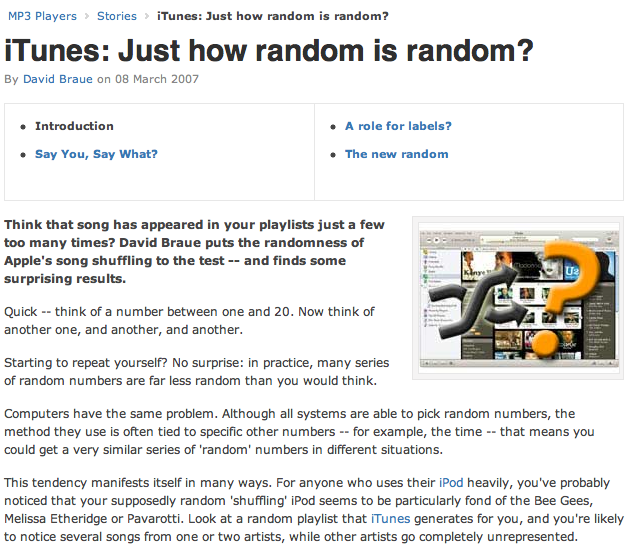
\includegraphics[width=\textwidth]{\chp3@path/3-1_define_probability/figures/iTunes}
\end{center}
\ct{ \webURL{http://www.cnet.com.au/itunes-just-how-random-is-random-339274094.htm}}
}

\end{frame}

%%%%%%%%%%%%%%%%%%%%%%%%%%%%%%%%%%%%

\begin{frame}
\frametitle{Probability}

\begin{itemize}

\item There are several possible interpretations of probability but they (almost) completely agree on the mathematical rules probability must follow.
\begin{itemize}
\item $P(A)$ = Probability of event A 
\item $0 \le P(A) \le 1$
\end{itemize}

\pause

\item \hl{Frequentist interpretation:} 
\begin{itemize}
\item The probability of an outcome is the proportion of times the outcome would occur if we observed the random process an infinite number of times.
\end{itemize}

\pause

\item \hl{Bayesian interpretation:} 
\begin{itemize}
\item  A Bayesian interprets probability as a subjective degree of belief: For the same event, two separate people could have different viewpoints and so assign different probabilities.
\item Largely popularized by revolutionary advance in computational technology and methods during the last twenty years.
\end{itemize}

\end{itemize}

\end{frame}

%%%%%%%%%%%%%%%%%%%%%%%%%%%%%%%%%%%%

% \begin{frame}
% \frametitle{Practice}

% \pq{Which of the following events would you be most surprised by?}

% \begin{enumerate}[(a)]
% \item exactly 3 heads in 10 coin flips
% \item exactly 3 heads in 100 coin flips
% \solnMult{exactly 3 heads in 1000 coin flips}
% \end{enumerate}

% \end{frame}

%%%%%%%%%%%%%%%%%%%%%%%%%%%%%%%%%%%%

\begin{frame}
\frametitle{Law of large numbers}

\hl{Law of large numbers} states that as more observations are collected, the proportion of occurrences with a particular outcome, \mathhl{\hat{p}_n}, converges to the probability of that outcome, \mathhl{p}.

\end{frame}

%%%%%%%%%%%%%%%%%%%%%%%%%%%%%%%%%%%%

\begin{frame}
\frametitle{Law of large numbers (cont.)}

\dq{When tossing a \textit{fair} coin, if heads comes up on each of the first 10 tosses, what do you think the chance is that another head will come up on the next toss? 0.5, less than 0.5, or more than 0.5?}

\[ \underline{H} \hspace{1mm} \underline{H} \hspace{1mm} \underline{H} \hspace{1mm} \underline{H} \hspace{1mm} \underline{H} \hspace{1mm} \underline{H} \hspace{1mm} \underline{H} \hspace{1mm} \underline{H} \hspace{1mm} \underline{H} \hspace{1mm} \underline{H} \hspace{1mm} \underline{?} \]

\begin{itemize}
\item<2-> The probability is still 0.5, or there is still a 50\% chance that another head will come up on the next toss.
\[ P(H \text{ on 11}^{th} \text{ toss}) = P(T \text{ on 11}^{th} \text{ toss}) = 0.5 \]
\item<3-> The coin is not ``due" for a tail.
\item<4-> The common misunderstanding of the LLN is that random processes are supposed to compensate for whatever happened in the past; this is just not true and is also called \hl{gambler's fallacy} (or \hl{law of averages}).
\end{itemize}

\end{frame}

%%%%%%%%%%%%%%%%%%%%%%%%%%%%%%%%%%%%

\section{Edfinity Quiz}

%%%%%%%%%%%%%%%%%%%%%%%%%%%%%%%%%%%%

\section{R Demo: LLN}

%%%%%%%%%%%%%%%%%%%%%%%%%%%%%%%%%%%%

\section{Edfinity Quiz}

%%%%%%%%%%%%%%%%%%%%%%%%%%%%%%%%%%%%

\subsection{Disjoint or mutually exclusive outcomes}

%%%%%%%%%%%%%%%%%%%%%%%%%%%%%%%%%%%%

\begin{frame}
\frametitle{Disjoint and non-disjoint outcomes}

\hl{Disjoint (mutually exclusive) outcomes:} Cannot happen at the same time.
\begin{itemize}
\item The outcome of a single coin toss cannot be a head and a tail.
\item A student both cannot fail and pass a class.
\item A single card drawn from a deck cannot be an ace and a queen.
\end{itemize}

\pause

\hl{Non-disjoint outcomes:} Can happen at the same time.
\begin{itemize}
\item A student can get an A in Stats and A in Econ in the same semester.
\end{itemize}

\end{frame}

%%%%%%%%%%%%%%%%%%%%%%%%%%%%%%%%%%%%

\begin{frame}
\frametitle{Union of non-disjoint events}

\dq{What is the probability of drawing a jack or a red card from a well shuffled full deck?}

\begin{figure}
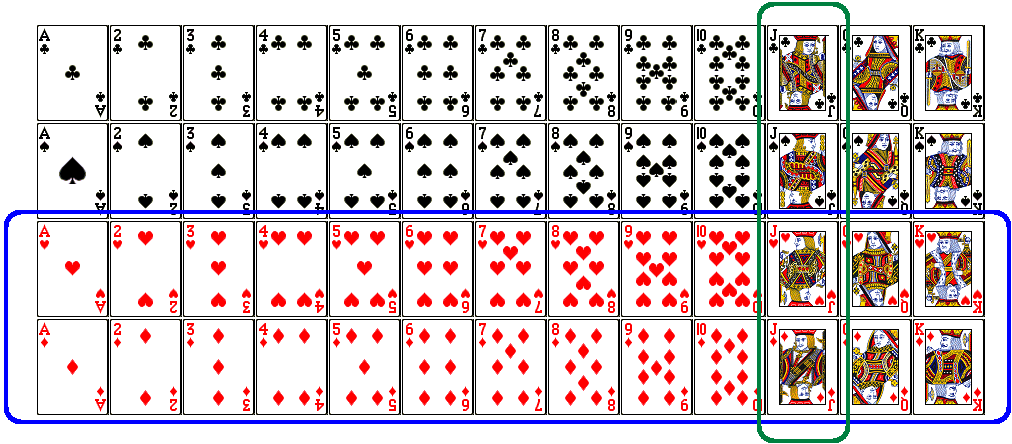
\includegraphics[width=0.7\textwidth]{\chp3@path/3-1_define_probability/figures/cards}
\end{figure}

\vspace{-0.75cm}

\soln{\onslide<2->{
\begin{align*}
P(jack~or~red) &= P(jack) + P(red) - \orange{$P(jack~and~red)$} \\
&= \frac{4}{52} + \frac{26}{52} - \frac{2}{52} = \frac{28}{52}
\end{align*}
}}

\vfill

\ct{Figure from \webURL{http://www.milefoot.com/math/discrete/counting/cardfreq.htm}.}

\end{frame}

%%%%%%%%%%%%%%%%%%%%%%%%%%%%%%%%%%%%

\subsection{Probabilities when events are not disjoint}

%%%%%%%%%%%%%%%%%%%%%%%%%%%%%%%%%%%%

% \begin{frame}
% \frametitle{Practice}

% \pq{What is the probability that a randomly sampled student thinks marijuana should be legalized \underline{or} they agree with their parents' political views?}

% {\small
% \begin{center}
% \begin{tabular}{l  cc c}
%             & \multicolumn{2}{c}{\textit{Share Parents' Politics}} & \\
% \cline{2-3}
% \textit{Legalize MJ} & No & Yes & Total \\
% \hline
% No          & 11 & 40 & 51 \\
% Yes         & 36 & 78 & 114 \\
% \hline
% Total       & 47 & 118 & 165
% \end{tabular}
% \end{center}
% }

% \begin{enumerate}[(a)]
% \item $\frac{40 + 36 - 78}{165}$
% \solnMult{$\frac{114 + 118 - 78}{165}$}
% \item $\frac{78}{165}$
% \item $\frac{78}{188}$
% \item $\frac{11}{47}$
% \end{enumerate}

% \end{frame}

%%%%%%%%%%%%%%%%%%%%%%%%%%%%%%%%%%%%

\section{Edfinity Quiz}

%%%%%%%%%%%%%%%%%%%%%%%%%%%%%%%%%%%%

\begin{frame}
\frametitle{Recap}

\formula{General addition rule}{\[ P(A~or~B) = P(A) + P(B) - P(A~and~B) \]}

\Note{For disjoint events $P(A~and~B) = 0$, so the above formula simplifies to $P(A~or~B) = P(A) + P(B)$.}

\end{frame}

%%%%%%%%%%%%%%%%%%%%%%%%%%%%%%%%%%%%

\subsection{Probability distributions}

%%%%%%%%%%%%%%%%%%%%%%%%%%%%%%%%%%%%

\begin{frame}
\frametitle{Probability distributions}

A \hl{probability distribution} lists all possible events and the probabilities with which they occur.

\begin{itemize}
\item The probability distribution for the gender of one kid:
{\footnotesize 
\begin{center}
\begin{tabular}{r | c | c}
Event    & Male		& Female \\
\hline
Probability	& 0.5		& 0.5 \\
\end{tabular}
\end{center}
}

\pause

\item Rules for probability distributions:
\begin{enumerate}
\item The events listed must be disjoint
\item Each probability must be between 0 and 1
\item The probabilities must total 1
\end{enumerate}

\pause

\item The probability distribution for the genders of two kids:
\soln{
\only<2->{
{\footnotesize
\begin{center}
\begin{tabular}{r | c | c | c | c}
Event		& MM	& FF		& MF		& FM \\
\hline
Probability	& 0.25	& 0.25	& 0.25	& 0.25 \\
\end{tabular}
\end{center}
}}}

\end{itemize}

\end{frame}

%%%%%%%%%%%%%%%%%%%%%%%%%%%%%%%%%%%%

% \begin{frame}
% \frametitle{Practice}

% \pq{In a survey, 52\% of respondents said they are Democrats. What is the probability that a randomly selected respondent from this sample is a Republican?}

% \begin{enumerate}[(a)]
% \item 0.48
% \item more than 0.48
% \item less than 0.48
% \solnMult{cannot calculate using only the information given}
% \end{enumerate}

% \soln{\only<2>{\orange{If the only two political parties are Republican and Democrat, then (a) is possible. However it is also possible that some people do not affiliate with a political party or affiliate with a party other than these two. Then (c) is also possible. However (b) is definitely not possible since it would result in the total probability for the sample space being above 1.}}}

% \end{frame}

%%%%%%%%%%%%%%%%%%%%%%%%%%%%%%%%%%%%

\subsection{Complement of an event}

%%%%%%%%%%%%%%%%%%%%%%%%%%%%%%%%%%%%

\begin{frame}
\frametitle{Sample space and complements}

\hl{Sample space} is the collection of all possible outcomes of a trial.

\begin{itemize}
\item A couple has one kid, what is the sample space for the gender of this kid? $S = \{ M, F \}$
\item A couple has two kids, what is the sample space for the gender of these kids? \soln{\pause{$S = \{ MM, FF, FM, MF \}$}}
\end{itemize}

\pause

\hl{Complementary events} are two mutually exclusive events whose probabilities that add up to 1.

\begin{itemize}
\item A couple has one kid. If we know that the kid is not a boy, what is gender of this kid?
\{ \sout{\textcolor{gray}{M}}, \orange{F} \} $\rightarrow$ Boy and girl are \hl{complementary} outcomes.
\item A couple has two kids, if we know that they are not both girls, what are the possible gender combinations for these kids?
\soln{\pause{\{ \orange{MM}, \sout{\textcolor{gray}{FF}}, \orange{FM}, \orange{MF} \} }}
\end{itemize}

\end{frame}

%%%%%%%%%%%%%%%%%%%%%%%%%%%%%%%%%%%%

\section{Edfinity Quiz}

%%%%%%%%%%%%%%%%%%%%%%%%%%%%%%%%%%%%

\subsection{Independence}

%%%%%%%%%%%%%%%%%%%%%%%%%%%%%%%%%%%%

\begin{frame}
\frametitle{Independence}

Two processes are \hl{independent} if knowing the outcome of one provides no useful information about the outcome of the other.

\pause

\begin{itemize}

\item Knowing that the coin landed on a head on the first toss \underline{does not} provide any useful information for determining what the coin will land on in the second toss. $\rightarrow$ Outcomes of two tosses of a coin are independent.

\pause

\item Knowing that the first card drawn from a deck is an ace \underline{does} provide useful information for determining the probability of drawing an ace in the second draw. $\rightarrow$ Outcomes of two draws from a deck of cards (without replacement) are dependent.

\end{itemize}

\end{frame}

%%%%%%%%%%%%%%%%%%%%%%%%%%%%%%%%%%%%

% \begin{frame}
% \frametitle{Practice}

% \pq{\small{Between January 9-12, 2013, SurveyUSA interviewed a random sample of 500 NC residents asking them whether they think widespread gun ownership protects law abiding citizens from crime, or makes society more dangerous. 58\% of all respondents said it protects citizens. 67\% of  White respondents, 28\% of Black respondents, and 64\% of Hispanic respondents shared this view. Which of the below is true?}}

% Opinion on gun ownership and race ethnicity are most likely
% \begin{enumerate}[(a)]
% \item complementary
% \item mutually exclusive
% \item independent
% \solnMult{dependent}
% \item disjoint
% \end{enumerate}

% \ct{\webURL{http://www.surveyusa.com/client/PollReport.aspx?g=a5f460ef-bba9-484b-8579-1101ea26421b}}

% \end{frame}

%%%%%%%%%%%%%%%%%%%%%%%%%%%%%%%%%%%%

\begin{frame}
\frametitle{}

\formula{Checking for independence}{If P(A occurs, given that B is true) = $P(A~|~B) = P(A)$, then A and B are independent.}

$\:$ \\

\soln{\pause{P(protects citizens) = 0.58 \\
\pause
$\:$ \\
P(randomly selected NC resident says gun ownership protects citizens, given that the resident is white) = \\ P(protects citizens $|$ White) = 0.67 \\
$\:$ \\
P(protects citizens $|$ Black) = 0.28 \\
$\:$ \\
P(protects citizens $|$ Hispanic) = 0.64 \\
$\:$ \\
\pause
P(protects citizens) varies by race/ethnicity, therefore opinion on gun ownership and race ethnicity are most likely dependent.
}}

\end{frame}

%%%%%%%%%%%%%%%%%%%%%%%%%%%%%%%%%%%%

\begin{frame}
\frametitle{Determining dependence based on sample data}

\begin{itemize}

\item If conditional probabilities calculated based on sample data suggest dependence between two variables, the next step is to conduct a hypothesis test to determine if the observed difference between the probabilities is likely or unlikely to have happened by chance.

\item If the observed difference between the conditional probabilities is large, then there is stronger evidence that the difference is real.

\item If a sample is large, then even a small difference can provide strong evidence of a real difference.

\end{itemize}

\pause

\dq{{\small We saw that P(protects citizens $|$ White) = 0.67 and P(protects citizens $|$ Hispanic) = 0.64. Under which condition would you be more convinced of a real difference between the proportions of Whites and Hispanics who think gun widespread gun ownership protects citizens? $n = 500$ or $n = 50,000$}} \pause \soln{$n = 50,000$}

\end{frame}

%%%%%%%%%%%%%%%%%%%%%%%%%%%%%%%%%%%%

\begin{frame}
\frametitle{}

\formula{Product rule for independent events}{\[P(A~and~B) = P(A) \times P(B) \]
\small{Or more generally, $P(A_1~and~\cdots~and~A_k) = P(A_1) \times \cdots \times P(A_k)$}}

\pause

\dq{You toss a coin twice, what is the probability of getting two tails in a row?}

\pause

\[ P(\text{T on the first toss}) \times  P(\text{T on the second toss}) = \frac{1}{2} \times \frac{1}{2} = \frac{1}{4} \]

\end{frame}

%%%%%%%%%%%%%%%%%%%%%%%%%%%%%%%%%%%%

% \begin{frame}
% \frametitle{Practice}

% \pq{A recent Gallup poll suggests that 25.5\% of Texans do not have health insurance as of June 2012. Assuming that the uninsured rate stayed constant, what is the probability that two randomly selected Texans are both uninsured?}

% \twocol{0.4}{0.6}
% {
% \begin{enumerate}[(a)]
% \item $25.5^2$
% \solnMult{ $0.255^2$ }
% \item $0.255 \times 2$
% \item $(1 - 0.255)^2$
% \end{enumerate}
% }
% {
% 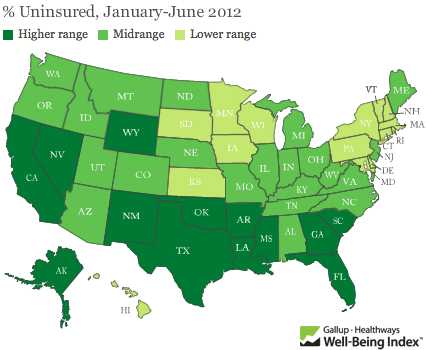
\includegraphics[width=0.9\textwidth]{\chp3@path/3-1_define_probability/figures/uninsured}
% }

% \ct{ \webURL{http://www.gallup.com/poll/156851/uninsured-rate-stable-across-states-far-2012.aspx}}

% \end{frame}

%%%%%%%%%%%%%%%%%%%%%%%%%%%%%%%%%%%%

\section{Edfinity Quiz}

%%%%%%%%%%%%%%%%%%%%%%%%%%%%%%%%%%%%

\subsection{Recap}

%%%%%%%%%%%%%%%%%%%%%%%%%%%%%%%%%%%%

\begin{frame}
\frametitle{Disjoint vs. complementary}

\dq{Do the sum of probabilities of two disjoint events always add up to 1?}

\pause

\soln{Not necessarily, there may be more than 2 events in the sample space, e.g. party affiliation.}

\pause
$\:$ \\

\dq{Do the sum of probabilities of two complementary events always add up to 1?}

\pause

\soln{Yes, that's the definition of complementary, e.g. heads and tails. }

\end{frame}

%%%%%%%%%%%%%%%%%%%%%%%%%%%%%%%%%%%%

\begin{frame}
\frametitle{Putting everything together...}

\dq{If we were to randomly select 5 Texans, what is the probability that at least one is uninsured?}

\begin{itemize}

\item If we were to randomly select 5 Texans, the sample space for the number of Texans who are uninsured would be:
\[ S = \{0, 1, 2, 3, 4, 5\} \]

\item We are interested in instances where at least one person is uninsured:
\[ S = \{0, \orange{$1, 2, 3, 4, 5$} \} \]

\item So we can divide up the sample space into two categories:
\[ S = \{0, \orange{at~least~one} \} \]

\end{itemize}

\end{frame}

%%%%%%%%%%%%%%%%%%%%%%%%%%%%%%%%%%%%

\begin{frame}
\frametitle{Putting everything together...}

Since the probability of the sample space must add up to 1:
\begin{eqnarray*}
Prob(at~least~1~uninsured) &=& 1 - Prob(none~uninsured) \\
\pause
&=& 1 - [(1-0.255)^5] \\
\pause
&=& 1- 0.745^5 \\
\pause
&=& 1 - 0.23 \\
\pause
&=& 0.77
\end{eqnarray*}

$\:$ \\
$\:$ \\

\formula{At least 1}{\[P(at~least~one) = 1 - P(none)\]}

\end{frame}

%%%%%%%%%%%%%%%%%%%%%%%%%%%%%%%%%%%%

% \begin{frame}
% \frametitle{Practice}

% \pq{Roughly 20\% of undergraduates at a university are vegetarian or vegan. What is the probability that, among a random sample of 3 undergraduates, at least one is vegetarian or vegan?}

% \twocol{0.3}{0.6}{
% \begin{enumerate}[(a)]
% \item $1 - 0.2 \times 3$
% \item $1 - 0.2^3$
% \item $0.8^3$
% \item $1 - 0.8 \times 3$
% \solnMult{$1 - 0.8^3$}
% \end{enumerate}
% }
% {
% \soln{ \only<2>{
% $P(at~least~1~from~veg) = 1- P(none~veg)$ \\
% $= 1 - (1 - 0.2)^3$ \\
% $= 1 - 0.8^3$ \\
% $= 1 - 0.512 = 0.488$ }}
% }

% \end{frame}

%%%%%%%%%%%%%%%%%%%%%%%%%%%%%%%%%%%%

%%%%%%%%%%%%%%%%%%%%%%%%%%%%%%%%%%%%
% End document
%%%%%%%%%%%%%%%%%%%%%%%%%%%%%%%%%%%%

\end{document}